% ============================================================
%  Capítulo 4: Resultados inferenciais
% ============================================================

\chapter{Resultados inferenciais}
\label{cap:resultados}

Este capítulo pergunta quais covariáveis acompanham a saída de um jogador da liga, posição por posição. Usamos três modelos. O Cox dá o efeito médio de cada covariável ao longo da carreira, e o diagnóstico de Schoenfeld mostra onde esse efeito médio deixa de valer. O Aalen mostra como o efeito se acumula com os anos, e o Cox--Aalen combina as duas leituras em um único ajuste. Lidos juntos, os modelos sustentam a leitura de cada posição, que fecha o capítulo.

% ─────────────────────────────────────────────────────────────
\section{Como os modelos foram ajustados}
\label{sec:res_procedimentos}

Cada jogador aparece em uma linha por temporada, e a saída é a última temporada do jogador na liga. O Cox com covariáveis dependentes do tempo (Capítulo~\ref{cap:metodologia}, Seção~\ref{sec:cox}) usa a experiência como tempo, e a seleção retroativa mantém as covariáveis com $p<0{,}05$. A experiência não entra como covariável, por ser o próprio tempo (Apêndice~\ref{subsec:apend_years_exp}). A forma linear e a colinearidade das listas finais estão no Apêndice~\ref{subsec:apend_forma}.

O Aalen não supõe proporcionalidade e estima o acréscimo acumulado de risco $\hat B(t)$ de cada covariável \citep{aalen1980}. Ele é lido só na faixa de anos em que a matriz de covariáveis tem posto completo. O teto de dez saídas por covariável \citep{harrell2001} se aplica ao total de saídas. Na janela de posto, o QB tem 72 saídas, cerca de 7 por covariável, e RB e WR têm mais de dez (Apêndice~\ref{subsec:apend_janela}). Os intervalos do Cox são os do erro-padrão do modelo, e a versão com variância robusta por jogador, usada como verificação, está no Apêndice~\ref{subsec:apend_robvar}. Os intervalos do Aalen usam a variância agrupada por jogador. O teste de média nula diz se o efeito médio é zero, mas não diz se ele muda; essa mudança se lê na forma de $\hat B(t)$. As covariáveis de carreira são defasadas até a temporada anterior, e as de temporada descrevem a própria temporada $t$, inclusive a última antes da saída. Por isso, os resultados se leem como associações e marcadores de risco, e cada HR é por desvio-padrão, com as demais covariáveis do modelo fixas.

O Cox e o Aalen são modelos de tempo contínuo, e aqui o tempo é anual: de 97\% a 99,7\% das saídas empatam com outra. Por isso, o Cox usa o método de Efron para os empates, e o Aalen trata as saídas de cada ano em bloco. Para verificar o Cox, ajustamos também o modelo de tempo discreto, um GLM binomial com ligação complementar log-log, que é a forma exata dos riscos proporcionais para tempo agrupado \citep{prentice1978}. O resultado bate com o Cox: nas três posições, nenhum termo final muda de sinal ou de significância a 5\%, e o HR da eficiência do QB é 0,64 contra 0,65, e o dos jogos perdidos do RB, 1,59 contra 1,55 (Apêndice~\ref{subsec:apend_empates}).

% ─────────────────────────────────────────────────────────────
\section{O efeito médio no Cox}
\label{sec:res_posicoes}

A Figura~\ref{fig:forest_cox} traz, para cada covariável do Cox final de cada posição, o HR por desvio-padrão (DP) e o intervalo de 95\%. Valor acima de 1 indica mais risco de saída, e abaixo de 1 indica menos.

No QB, a fatia de passes da equipe tem o maior efeito em HR: um DP dela, cerca de 39 pontos percentuais, corresponde a cerca de 71\% menos risco estimado. A eficiência de passe é o sinal mais estável. Um QB 21 pontos de \textit{passer rating} acima da média, cerca de um DP, tem cerca de 35\% menos risco estimado de sair naquela temporada. A eficiência tem sinal negativo com $p<0{,}001$ nos três modelos, e está entre as duas covariáveis de maior queda do $C$ por permutação em cada modelo preditivo (Tabela~\ref{tab:tgb_imp_inf}). A produção por passe também pesa: um DP de TD\% histórico (cerca de 1 ponto percentual) corresponde a cerca de 37\% menos risco. Na direção contrária, com a fatia de passes no modelo, a participação ofensiva do jogador se associa a mais risco: um DP dela, cerca de 33 pontos percentuais, corresponde a cerca de 71\% mais risco (Apêndice~\ref{subsec:apend_forma}). Quem tem até 50 passes observados na janela, até a temporada anterior, também sai mais: a passagem do indicador de 0 para 1 corresponde a um HR de $1{,}82$, ou seja, cerca de 82\% mais risco estimado. O HR por desvio-padrão dessa covariável, de $1{,}31$, está na Figura~\ref{fig:forest_cox}.

No RB, a disponibilidade e a fatia de jardas terrestres da equipe são os dois sinais mais fortes. Cada desvio-padrão de jogos perdidos, cerca de cinco jogos, corresponde a cerca de 55\% mais risco estimado de não voltar. O termo tem $p<0{,}001$ nos três modelos e é o de maior queda do $C$ por permutação em cada modelo preditivo (Tabela~\ref{tab:tgb_imp_inf}). A fatia de jardas tem sentido oposto, e o maior efeito em HR: um DP dela, cerca de 22 pontos percentuais, corresponde a cerca de metade do risco. Cada degrau para baixo no \textit{depth chart} corresponde a cerca de 23\% mais risco, controlando as demais covariáveis, inclusive as ausências (razão de riscos de $1{,}23$ por degrau; $1{,}17$ por desvio-padrão, que vale $0{,}75$ degrau). A eficiência de corrida acumulada na carreira, medida pelas jardas por corrida até a temporada anterior, está associada a menor risco: um DP, cerca de meia jarda por corrida, corresponde a cerca de 18\% menos risco.

\begin{figure}[H]
\centering
\thesisfigpanel{a}{\thesisfigforestcompact}{figuras/forest_plot_QB.pdf}
\thesisfigpanel{b}{\thesisfigforestcompact}{figuras/forest_plot_RB.pdf}
\thesisfigpanel{c}{\thesisfigforestcompact}{figuras/forest_plot_WR.pdf}
\caption{HR por desvio-padrão (DP) e IC de 95\% de cada covariável do Cox final, por posição, em escala log. HR acima de 1 (laranja): um DP a mais está associado a mais risco de saída; abaixo de 1 (verde), a menos. Tracejado: HR = 1, sem associação. (a) QB; (b) RB; (c) WR.}
\label{fig:forest_cox}
\end{figure}

No WR, o papel de alvo principal é o sinal de maior magnitude em HR, e está ligado a menor risco nos três modelos. Um DP de fatia de alvos da equipe, cerca de 9 pontos percentuais, corresponde a cerca de 73\% menos risco, o que dá cerca de metade do risco a cada 5 pontos percentuais. A idade se associa a mais risco: um WR três anos mais velho tem cerca de 69\% mais risco estimado. Cinco jogos perdidos a mais numa temporada correspondem a cerca de 27\% mais risco, e cem jardas a mais de corrida históricas, a cerca de 15\% menos. A altura também pesa, com um DP (cerca de 6 cm) ligado a cerca de 13\% mais risco.


\subsection{Onde a proporcionalidade não se sustenta}
\label{subsec:schoenfeld}

Um HR único só resume bem a carreira inteira se o efeito for o mesmo em todos os anos. O teste de Schoenfeld verifica isso para cada covariável, e a Tabela~\ref{tab:schoenfeld} traz o teste global e o de cada termo do RB e do WR. No QB, o teste global não rejeita ($p=0{,}201$), e nenhum termo rejeita, de modo que não há evidência contra um HR único.

\begin{table}[H]
\centering
\caption{Teste de Schoenfeld do Cox final para RB e WR: $\chi^2$, gl e valor-$p$ de cada covariável e do teste global. Valor-$p$ abaixo de $0{,}05$ rejeita efeito constante no tempo.}
\label{tab:schoenfeld}
\thesistablesetup
\begin{tabularx}{\textwidth}{@{}>{\raggedright\arraybackslash}Xrrr@{}}
\toprule
\textbf{Covariável} & \textbf{$\chi^2$} & \textbf{gl} & \textbf{$p$} \\
\midrule
\multicolumn{4}{@{}l}{\textbf{Running backs}} \\
Jogos perdidos                      & $10{,}60$ & 1 & $0{,}001$ \\
Fatia de jardas terrestres          & $9{,}78$  & 1 & $0{,}002$ \\
Profundidade no elenco              & $0{,}77$  & 1 & $0{,}381$ \\
Posição no \textit{draft}              & $0{,}00$  & 1 & $0{,}963$ \\
Hist. defasado YPC                  & $0{,}27$  & 1 & $0{,}604$ \\
\textbf{Global}                     & $\mathbf{12{,}79}$ & $\mathbf{5}$ & $\mathbf{0{,}025}$ \\
\midrule
\multicolumn{4}{@{}l}{\textbf{Wide receivers}} \\
Jogos perdidos                      & $10{,}86$ & 1 & $0{,}001$ \\
Fatia de alvos                      & $7{,}39$  & 1 & $0{,}007$ \\
Hist. defasado de jardas de corrida & $3{,}71$  & 1 & $0{,}054$ \\
Hist. defasado alvos na \textit{red zone} & $1{,}51$ & 1 & $0{,}219$ \\
Participação ofensiva               & $1{,}26$  & 1 & $0{,}261$ \\
Idade                               & $0{,}08$  & 1 & $0{,}774$ \\
Altura                              & $0{,}03$  & 1 & $0{,}867$ \\
\textbf{Global}                     & $\mathbf{15{,}39}$ & $\mathbf{7}$ & $\mathbf{0{,}031}$ \\
\bottomrule
\end{tabularx}
\end{table}

No RB, o teste global rejeita ($p=0{,}025$), e a rejeição vem de dois termos: os jogos perdidos e a fatia de jardas terrestres. A inclinação de $\beta(t)$ contra o tempo é negativa nas ausências e positiva na fatia, ou seja, em razão de riscos os dois efeitos se aproximam de 1 com os anos. O HR de cada um é, portanto, a média de um efeito que enfraquece. No WR, o mesmo acontece com as ausências e com a fatia de alvos, e o teste global rejeita ($p=0{,}031$). Quando o teste rejeita, o HR é uma média, e o Aalen, que não supõe proporcionalidade, mostra a forma dessa mudança.

% ─────────────────────────────────────────────────────────────
\section{O Aalen: como o efeito se acumula}
\label{sec:aalen_res}

Enquanto o Cox estima um único coeficiente com a informação de todos os anos, o Aalen estima um incremento em cada ano de carreira. Ele é lido só nos anos em que o conjunto é estimável: até o 11º ano no QB, o 9º no RB e o 10º no WR.

\begin{figure}[H]
\centering
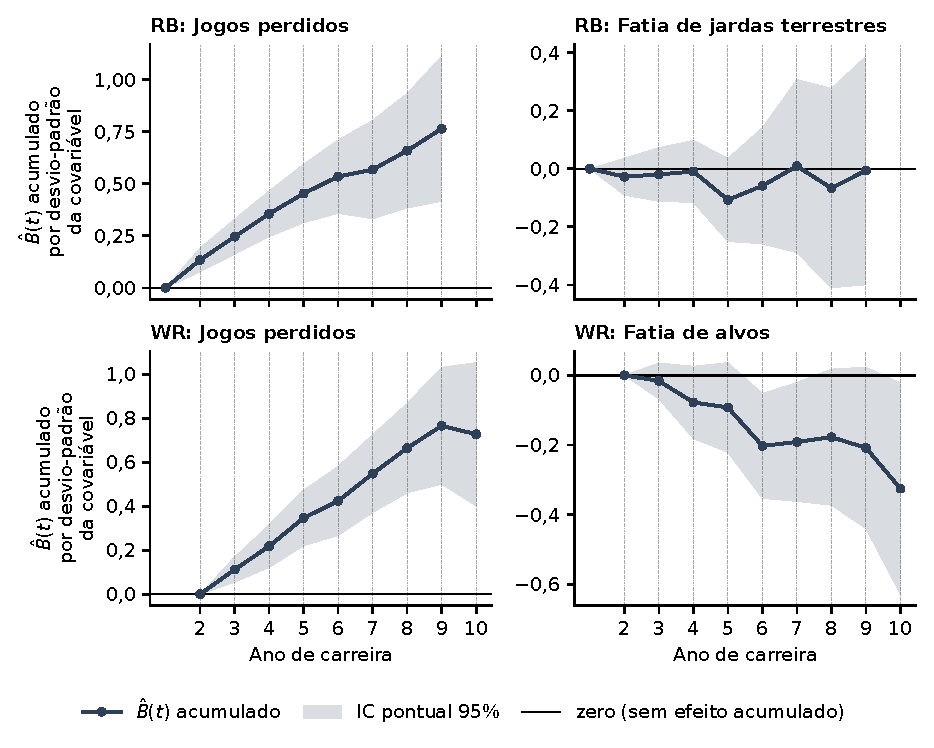
\includegraphics[width=0.86\textwidth]{figuras/aalen_termos_violacao.pdf}
\caption{$\hat B(t)$ acumulado do Aalen por ano de carreira, em RB (jogos perdidos, fatia de jardas) e WR (jogos perdidos, fatia de alvos). A inclinação mostra quanto risco um DP da covariável soma em cada ano: subida, mais risco; descida, menos; reta, acréscimo constante. Linha em zero: sem efeito acumulado. Faixa cinza: IC 95\%, variância robusta por jogador.}
\label{fig:aalen_viol}
\end{figure}

No QB, o risco acumulado associado à eficiência de passe desce de forma regular, chegando a cerca de $-0{,}21$ no 5º ano e $-0{,}61$ no 10º, por desvio-padrão. No WR, a idade soma risco acumulado, e a fatia de alvos o reduz.

No RB, o risco acumulado de ausências sobe quase em linha reta: do 2º ao 9º ano, um desvio-padrão a mais de jogos perdidos na temporada soma em média cerca de 0,1 ao risco do ano, e a soma chega a cerca de 0,76 no 9º ano (Figura~\ref{fig:aalen_viol}, painel superior esquerdo). Como o tempo é anual, cada incremento se lê como diferença de probabilidade de saída naquele ano: 0,1 equivale a cerca de 10 pontos percentuais. A curva soma esses incrementos e não é uma probabilidade nem uma razão de riscos. O desenho é compatível com um acréscimo constante. A fatia de jardas terrestres não tem trajetória definida: oscila perto de zero e o intervalo contém zero em todos os anos, de modo que não serve como critério de risco nesta leitura.

No WR, as ausências seguem o mesmo padrão quase linear entre o 3º e o 9º ano, com intervalo que exclui zero desde o 3º ano. A curva da fatia de alvos desce sobretudo até o 6º ano e depois fica em patamar, e o intervalo só exclui zero nos anos 6, 7 e 10. No 10º ano, a queda se apoia em 52 linhas em risco e 10 saídas.


% ─────────────────────────────────────────────────────────────
\section{O híbrido Cox--Aalen}
\label{sec:res_coxaalen}

O modelo de \citet{scheike2002} junta as duas leituras em um único ajuste. As covariáveis que o Schoenfeld marcou entram com efeito acumulado $\hat B(t)$, e as demais entram com HR constante, como no Cox. No QB, nenhuma covariável foi marcada, e todas ficam no bloco multiplicativo: o híbrido é o próprio Cox, e as diferenças vêm da implementação. No RB e no WR, o bloco aditivo recebe jogos perdidos e a fatia da equipe (jardas terrestres no RB, alvos no WR). A ordem das saídas dentro de cada ano está no Apêndice~\ref{subsec:apend_cox_aalen}.

No RB, o efeito de jogos perdidos no bloco aditivo cresce quase em linha reta: o teste não rejeita a constância ($p=0{,}847$). No mesmo bloco, a fatia de jardas está associada a menor risco ($p=0{,}003$ no teste de média nula), e o teste não rejeita a constância ($p=0{,}509$), o que é compatível com um declínio linear, sem comprová-lo. O Aalen final não a separa de zero ($p=0{,}523$); com a lista do Cox, que não tem a participação ofensiva nem outros três termos, ele também separa a fatia ($p=0{,}016$), de modo que a diferença vem do conjunto de covariáveis. Por isso a fatia de jardas fica como sinal a acompanhar. No WR, a fatia de alvos e as ausências seguem o sentido do Aalen final, e o teste também não rejeita a constância ($p=0{,}474$ e $p=0{,}863$). Nos dois casos, o híbrido completa o Schoenfeld: com o bloco multiplicativo na média, os dados são compatíveis com um acréscimo constante por ano, e na razão de riscos o efeito enfraquece.

% ─────────────────────────────────────────────────────────────
\section{Os três modelos lado a lado}
\label{sec:res_lado}

\begin{table}[H]
\centering
\caption{Sinal ($+$ mais risco, $-$ menos, $\approx 0$ nulo) e valor-$p$ de cada covariável no Cox, no Aalen e no Cox--Aalen finais, por posição. Célula vazia: covariável fora do modelo.}
\label{tab:concordancia}
\thesistablesetup
\footnotesize
\begin{tabularx}{\textwidth}{@{}>{\raggedright\arraybackslash}Xccc@{}}
\toprule
\textbf{Covariável} & \textbf{Cox} & \textbf{Aalen} & \textbf{Cox--Aalen} \\
\midrule
\multicolumn{4}{@{}l}{\textbf{Quarterbacks}} \\
Eficiência de passe            & $-$; $<0{,}001$ & $-$; $<0{,}001$ & $-$; $<0{,}001$ \\
Fatia de passes                & $-$; $<0{,}001$ & $-$; $0{,}024$  & $-$; $<0{,}001$ \\
Participação ofensiva          & $+$; $<0{,}001$ & $+$; $0{,}022$  & $+$; $<0{,}001$ \\
Hist. defasado TD\%            & $-$; $<0{,}001$  & $-$; $0{,}122$  & $-$; $<0{,}001$ \\
Hist. defasado comp\% ausente  & $+$; $0{,}036$  & & $+$; $0{,}006$  \\
Posição no \textit{draft}      & & $+$; $0{,}029$  & \\
\midrule
\multicolumn{4}{@{}l}{\textbf{Running backs}} \\
Jogos perdidos                 & $+$; $<0{,}001$ & $+$; $<0{,}001$ & $+$; $<0{,}001$ (aditivo) \\
Fatia de jardas terrestres     & $-$; $<0{,}001$ & $-$; $0{,}523$  & $-$; $0{,}003$ (aditivo) \\
Profundidade no elenco         & $+$; $0{,}028$  & $+$; $0{,}013$  & $+$; $0{,}009$  \\
Posição no \textit{draft}      & $+$; $0{,}039$  & $+$; $0{,}272$  & $+$; $0{,}201$  \\
Hist. defasado YPC             & $-$; $0{,}002$  & $-$; $0{,}010$  & $-$; $0{,}012$  \\
\midrule
\multicolumn{4}{@{}l}{\textbf{Wide receivers}} \\
Jogos perdidos                 & $+$; $0{,}013$  & $+$; $<0{,}001$ & $+$; $<0{,}001$ (aditivo) \\
Idade                          & $+$; $0{,}003$  & $+$; $0{,}005$  & $+$; $0{,}029$  \\
Altura                         & $+$; $0{,}022$  & & $+$; $0{,}024$  \\
Hist. defasado de jardas de corrida & $-$; $0{,}029$ & $-$; $<0{,}001$ & $-$; $0{,}063$ \\
Hist. defasado de alvos na \textit{red zone} & $-$; $0{,}007$ & $-$; $0{,}062$ & $-$; $<0{,}001$ \\
Participação ofensiva          & $+$; $0{,}026$  & $\approx 0$; $0{,}948$ & $\approx 0$; $0{,}924$ \\
Fatia de alvos                 & $-$; $<0{,}001$ & $-$; $0{,}021$  & $-$; $0{,}008$ (aditivo) \\
Não draftado                   & & $-$; $0{,}019$  & \\
\bottomrule
\end{tabularx}
\end{table}

A Tabela~\ref{tab:concordancia} junta as três leituras, com as covariáveis do Cox final e as que o Aalen separa de zero a 5\%. No Aalen e no bloco aditivo do híbrido, o $p$ é do teste de média nula; no Cox e no bloco multiplicativo, do teste de Wald.


\subsection{Onde os modelos discordam, e por quê}
\label{subsec:divergencias}

Onde os três modelos concordam, a conclusão se sustenta: nove termos têm sinal e significância a 5\% nos três, listados na síntese deste capítulo. Nas demais covariáveis, a discordância tem três fontes. A primeira é que o Cox dá uma média, enquanto o Aalen e o híbrido mostram o efeito ao longo dos anos, e um HR único pode estar correto como média e ainda esconder essa variação. A segunda é o suporte: a janela do Aalen tem menos saídas que o Cox. A terceira é o conjunto de covariáveis que acompanha cada termo. A \textit{red zone} do WR tem $p=0{,}062$ no Aalen, onde compete com outras 12 covariáveis, e $p<0{,}001$ no híbrido, onde compete só com as multiplicativas.


% ─────────────────────────────────────────────────────────────
\section{Leitura por posição}
\label{sec:res_leitura}

\subsection{Quarterbacks}
\label{subsec:qb}

Para o QB, o que pesa é a produção em campo. A eficiência de passe é significativa nos três modelos, com $p<0{,}001$ em todos, e é o sinal mais firme. A fatia de passes tem sinal negativo nos três. O TD\% histórico segue o mesmo sentido no Cox e no híbrido, e o Aalen não o separa de zero ($p=0{,}122$). A participação ofensiva, lida com a fatia no modelo, tem sinal positivo nos três. A posição no \textit{draft} aparece apenas no Aalen ($p=0{,}029$).

\subsection{Running backs}
\label{subsec:rb}

Para o RB, a disponibilidade é o termo que mais pesa na permutação e no Aalen. A leitura útil é o acréscimo anual, de cerca de 0,1, e não o HR único. A hierarquia do elenco também conta, e um RB que desce no \textit{depth chart} tem mais risco, no Aalen ($p=0{,}013$) e no híbrido ($p=0{,}009$). A fatia de jardas da equipe está associada a menor risco, mas sua força depende do modelo: o Aalen não a distingue de zero, e o híbrido a separa com clareza. A posição no \textit{draft} só é significativa no Cox, com HR de $1{,}12$ por desvio-padrão, e no híbrido não se distingue de zero ($p=0{,}201$). Sem as covariáveis de uso, a posição no \textit{draft} tem HR de $1{,}58$, e os não draftados, de $1{,}46$.

\subsection{Wide receivers}
\label{subsec:wr}

Para o WR, quem concentra alvos tende a permanecer. A idade e as ausências formam o outro lado. A idade se associa a mais risco nos três modelos ($p=0{,}003$, $0{,}005$ e $0{,}029$), e os jogos perdidos seguem o mesmo sentido. As jardas de corrida históricas são significativas no Cox e no Aalen, mas têm $p=0{,}063$ no híbrido, e a \textit{red zone} não se distingue de zero no Aalen. A participação ofensiva tem sinal positivo no Cox ($p=0{,}026$) e perde o sinal no Aalen e no híbrido ($p=0{,}948$ e $p=0{,}924$). Como a experiência é o eixo do tempo, o efeito da idade é o da idade de entrada na liga, e não o do envelhecimento dentro da carreira.

% ─────────────────────────────────────────────────────────────
\section{Síntese da parte inferencial}
\label{sec:sintese_inferencial}

Nove associações têm $p<0{,}05$ nos três ajustes, de modo que o seu sentido não depende da escala do modelo: no QB, a eficiência de passe, a fatia de passes e a participação ofensiva; no RB, as ausências, a profundidade no elenco e a eficiência de corrida; no WR, as ausências, a idade e a fatia de alvos. As covariáveis fora das nove são sinais a acompanhar.
